\section{Tuning methods}
Different methods can be used to tune a PID controller as the, Zieggler-Nichols, Skogestad and Good Gain method, having in common the same goal : Get a fast response and provide a good stability.\par
As a first try, a PID controller was designed using the Good Gain method. Later, a comparison between P, PI, PD and PID controllers was performed with the \emph{PID Simulink} box, in order to choose the most effective one for our application.\par 	

\subsubsection{The Good Gain}


Can be seen on the figure below, the structure of the controller. Taking as input the error angle \textbf{$\theta_{e}$} and outputting the required voltage \textit{V}, which is after limited by a saturation box to supply the motor, this controller has the final task of converting a value in radian into voltage.\par

\begin{figure}[H]
  \centering
  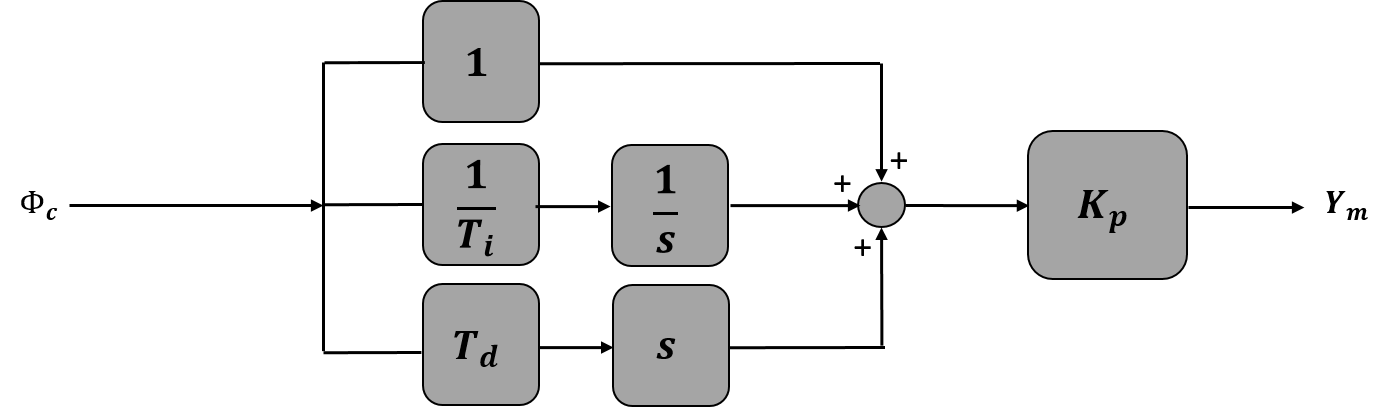
\includegraphics[scale=0.5]{figures/controller_model.png}
  \caption[LABEL] {Block diagram of the PID controller}
\end{figure}
  

  
    
The steps of the experiment based method, the Good Gain, are the followings :\par 

 This method can be split in three different parts. In the first part it is supposed to set the proportional parameter. Thus, by choosing in the step from the figure \ref{fig:subim11} , $T_i$ = $\infty$ and $T_d$ = 0, it sets respectively the integral and the derivative term to zero.

\begin{figure}[H]
\hfill
\subfigure[Set Ti = inf , Td = 0 and Kp = 1]{
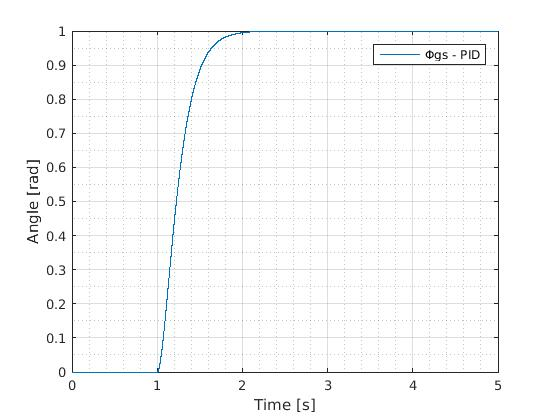
\includegraphics[scale=0.3]{figures/GG1.jpg}
\label{fig:subim11}}
\hfill
\subfigure[Increase Kp until finding a slight overshoot but a well damped response]{
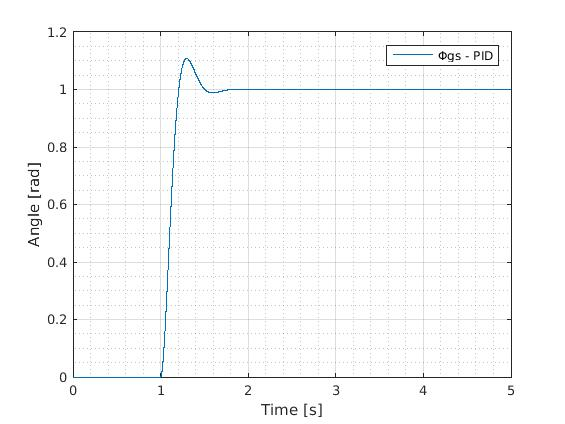
\includegraphics[scale=0.3]{figures/GG2.jpg}
\label{fig:subim12}}

\caption{Good Gain : Setting the propotional parameter}
\end{figure}


Increasing $K_p$ in figure \ref{fig:subim12} will allow to reduce the rising time. Morover, changing this proportional gain is a needed step to find a slight overshoot and a well damped response. Hence, having an overshoot and the first undershoot, $T_{out}$ can be defined, being the time between the peak of the overshoot and the one of the undershoot.\par
\vspace{5mm}
Adding the integral parameter imply a relation with the previous defined time between the peak of the overshoot and undershoot. Thus, $T_i = 1.5 * T_{out}$. The objective of this step \ref{fig:subim13} is to eliminate the steady state error.



\begin{figure}[H]
\hfill
\subfigure[Set Ti = 1.5$\cdot T_{out}$]{
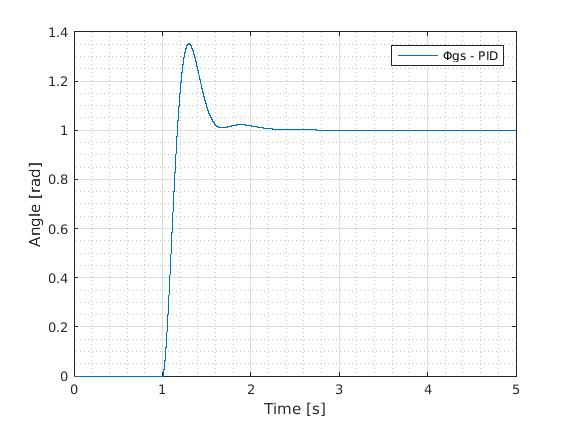
\includegraphics[scale=0.29]{figures/GG3.jpg}
\label{fig:subim13}}
\hfill
\subfigure[Set Td = $\frac{Ti}{4}$]{
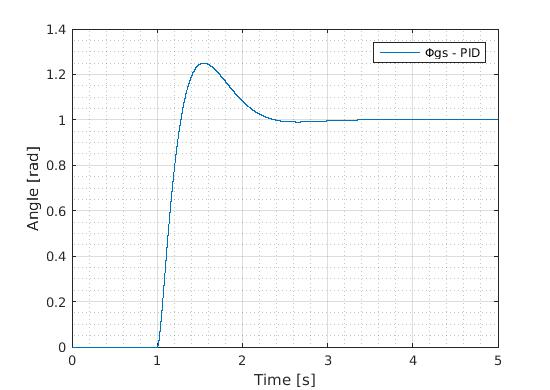
\includegraphics[scale=0.31]{figures/GG4.jpg}
\label{fig:subim14}}
\hfill

\caption{Good Gain : Adding integral and derivative parts}
\end{figure}

At this point, the controller is a proportional-integral. The high overshoot resulting from adding the integral term can be attenuated by setting the derivative part, shown in figure \ref{fig:subim14}. The gain $T_d$ will act as a damper on the system and therefore reduce the high variations of the step response. In the Good Gain method, this value is described to be $T_d = \frac{T_i}{4}$.

\vspace{5mm}

Theoretically, the tuning of the controller using the Good Gain method is done. However, it is possible to improve the controller based on the application that is wanted. In the case of this project, stability and minor overshoot was more important than the reaching speed of the reference value. Therefore, based on the principles seen in sections \ref{sec:pid_theory}, the overshoot of the system was attenuated, the undershoot cancelled and the drop-off smoothed (figure \ref{finalGG}).

\begin{figure}[H]
  \centering
  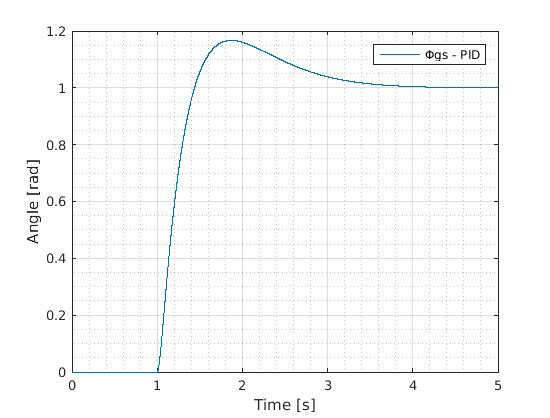
\includegraphics[scale=0.5]{figures/GG5.jpg}
  \caption[LABEL] {Good Gain : final settings}
  \label{finalGG}
\end{figure}


  
\subsubsection{PID Simulink box}
\begin{figure}[H]
\centering
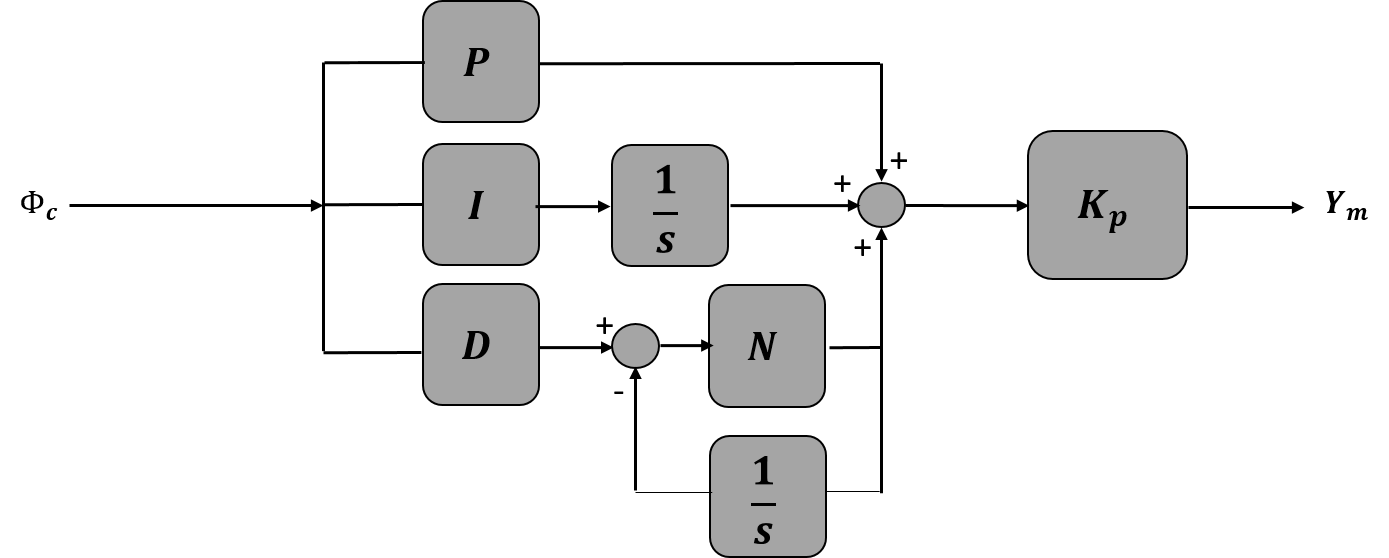
\includegraphics[scale=0.4]{figures/controller_box.png}
\caption{Inside of the PID box}
\label{dcmotor_circuit}
\end{figure}

\begin{figure}[H]
\centering
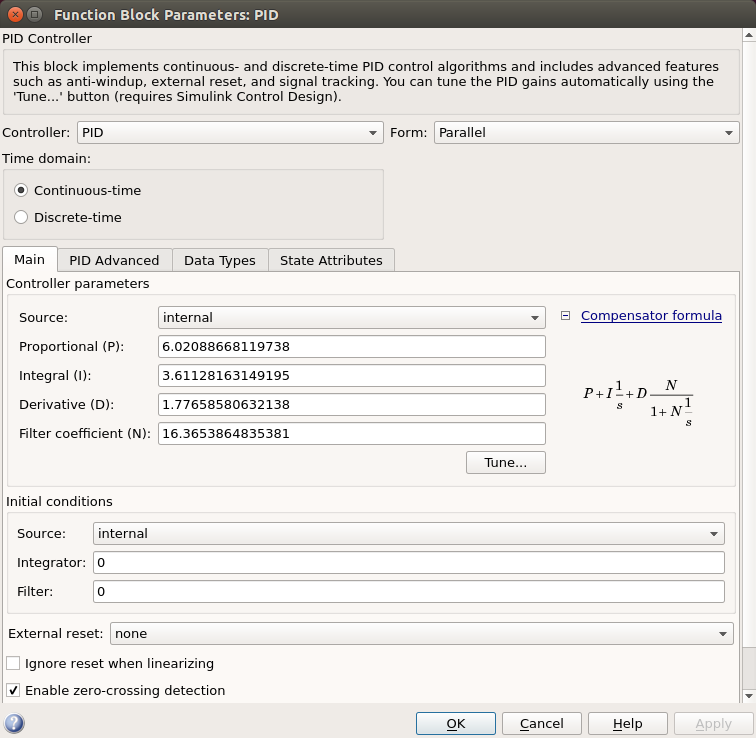
\includegraphics[scale=0.4]{figures/PID_window.png}
\caption{Inside of the PID box}
\label{dcmotor_circuit}
\end{figure}


\begin{figure}[H]
\centering
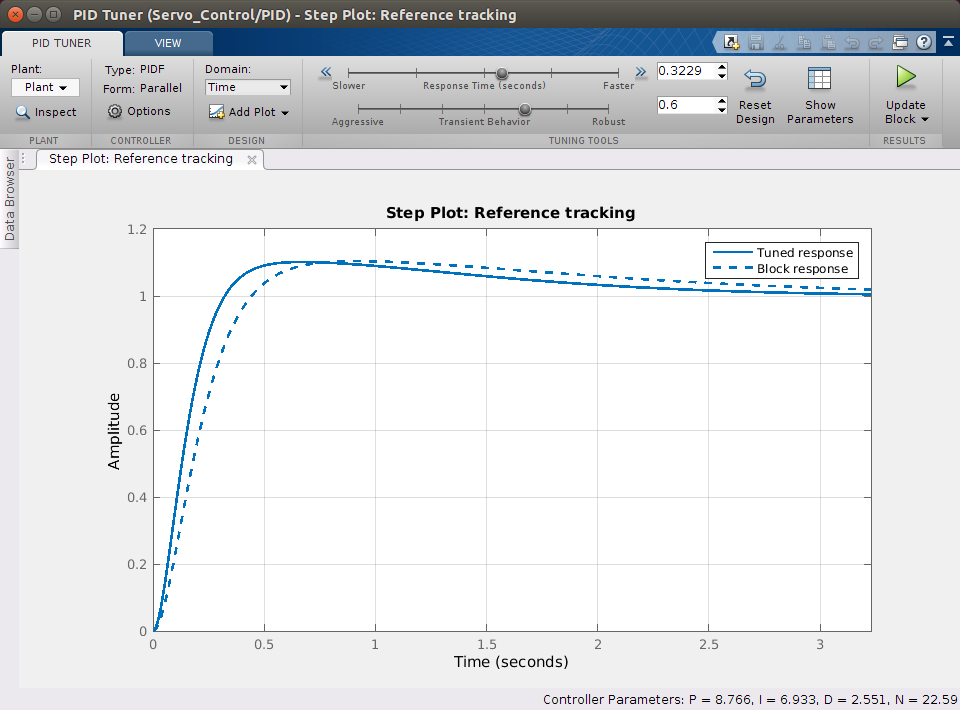
\includegraphics[scale=0.4]{figures/PID_param.png}
\caption{Tuning tool of the PID box}
\label{dcmotor_circuit}
\end{figure}
  


